\documentclass[12pt]{article}
\usepackage[utf8]{inputenc}
\usepackage[T1]{fontenc}
\usepackage{hyperref}
\usepackage{lipsum} % for placeholder text, remove if not needed
\usepackage[a4paper, portrait, margin=1.5cm]{geometry}
\usepackage{graphicx}
\usepackage{fancyhdr}
\usepackage{float}
\usepackage{color}
\usepackage{subcaption}


\title{IBM AI AR techdoc}
\author{Ani Bitri}


\begin{document}
% \supervisor{Dr. Paris Giampouras, John McNamara}

\maketitle
\tableofcontents
\newpage

\section{Requirements}
Each requirement will be described in the format R{n}C/D, where n is the requirement number and C or D indicates whether the requirement is customer (C) or developer (D) oriented. For example,
R1C refers to the first customer requirement, while R2D refers to the second developer requirement. Each requirement will be detailed with its description, priority, verification method and traceability.

    \subsection{Functional Requirements}
    List the key functionalities the software system must support. Provide clear and concise descriptions of features and interactions.

    \begin{enumerate}
        \item \textbf{Augmented Reality System}
    \end{enumerate}

    \subsection{Non-Functional Requirements}
    Outline performance, usability, reliability, and other quality attributes expected from the system.

\section{System Architecture}
Provide a high-level overview of the system architecture. Include diagrams where appropriate to illustrate the system components and their interactions.

    \subsection{Design Pattern}

    The design pattern which will be adopted for this project is the Model-View-ViewModel (MVVM) pattern. This pattern is well-suited for applications that require a clear separation
    of concerns between the user interface and logic, making it easier to manage and test the application. Furthermore, the MVVM pattern facilitates a more modular and maintainable
    codebase, which is essential for the iterative development process planned for this project. The image below illustrates the MVVM architecture which will be used in the project.

    \begin{figure}[H]
        \centering
        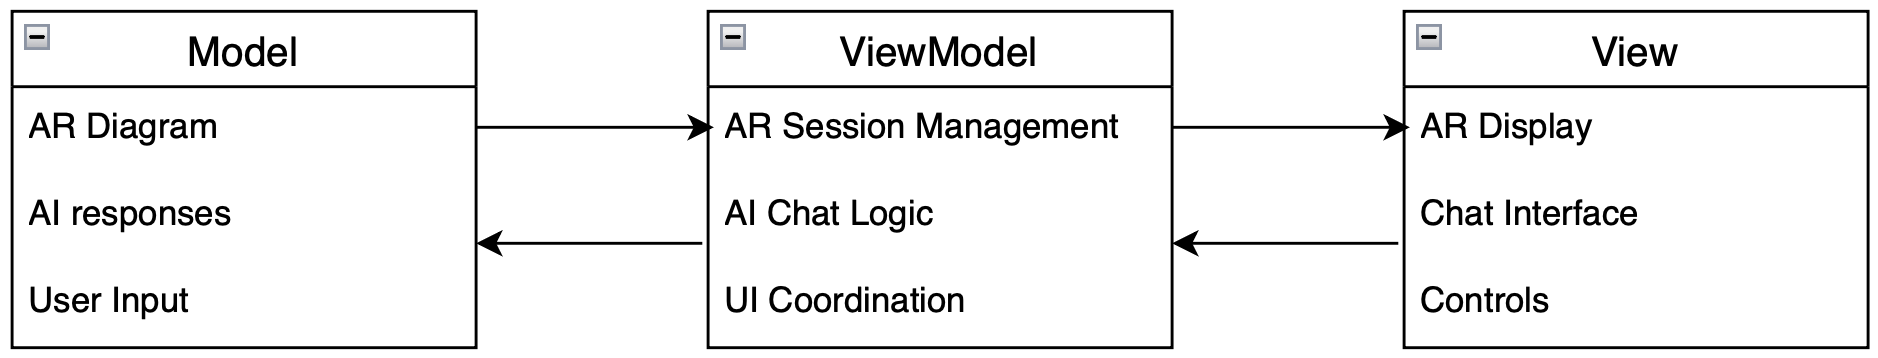
\includegraphics[width=\textwidth]{img/Pattern.png}
        \caption{MVVM Architecture Pattern}
        \label{fig:Pattern}
    \end{figure}

    \subsection{Frontend Design}

    \subsubsection{User Interface and User Experience}

        The application will feature a user-friendly interface that allows users to easily navigate through the app and access its features. The UI will be designed to be intuitive and responsive, ensuring a seamless user experience. When the user open the app, they will be presented with
        a simple home screen with options to scan a document, upload a document or access the history of previously scanned documents. Besides the home screen, the app will also include a tab for the chatbot, where users can interact with the AI assistant, and a settings tab for configuring
        app preferences. The image below illustrates the proposed UI design for the application:

        \begin{figure}
            \centering
            \begin{subfigure}{0.3\textwidth}
                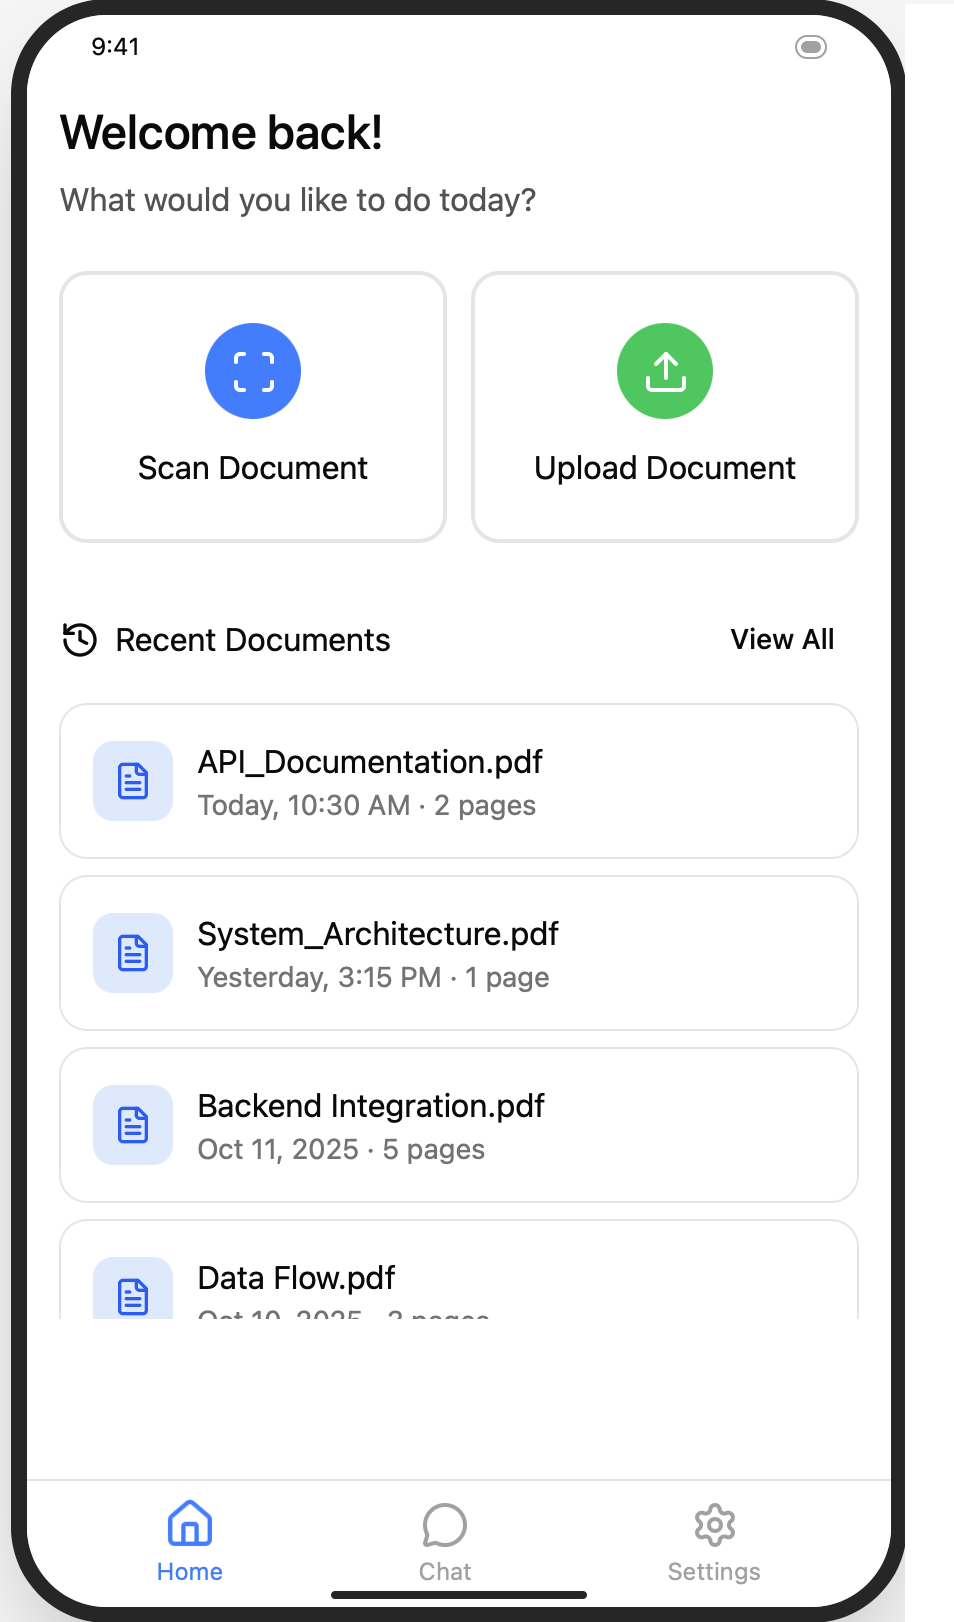
\includegraphics[width=\textwidth]{img/FrontendHomeTab.png}
                \caption{Home Screen}
                \label{fig:HomeScreen}
            \end{subfigure}
            \hfill
            \begin{subfigure}{0.3\textwidth}
                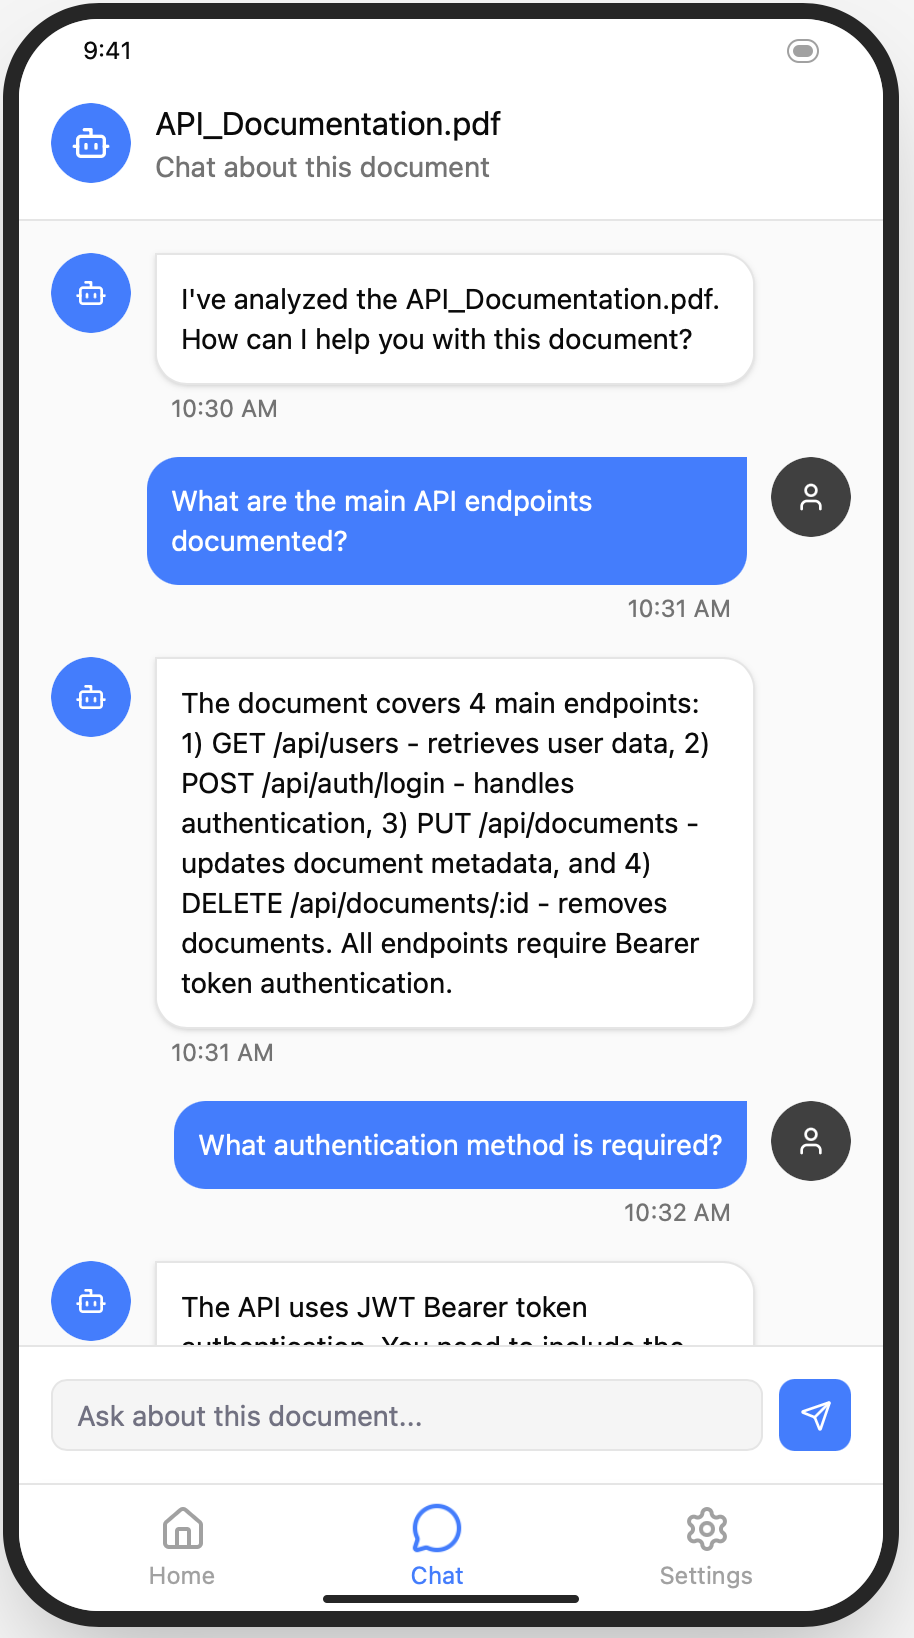
\includegraphics[width=\textwidth]{img/FrontendChatTab.png}
                \caption{Chatbot Tab}
                \label{fig:ChatbotTab}
            \end{subfigure}
            \hfill
            \begin{subfigure}{0.3\textwidth}
                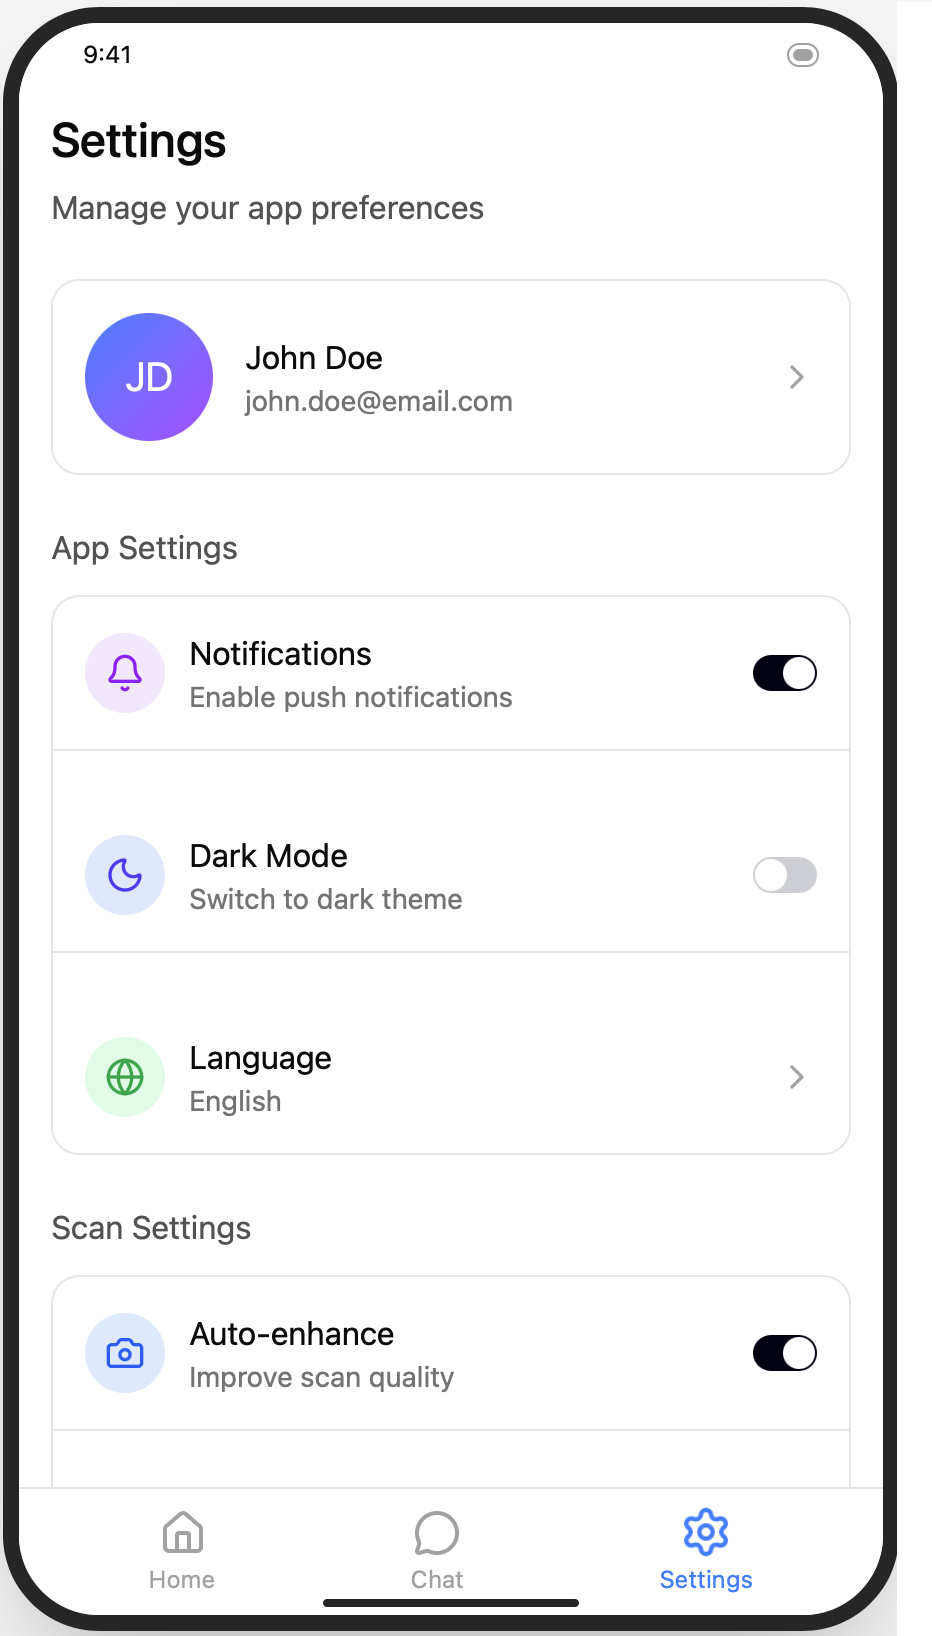
\includegraphics[width=\textwidth]{img/FrontendSettingsTab.png}
                \caption{Settings Tab}
                \label{fig:SettingsTab}
            \end{subfigure}
            \caption{Proposed UI Design for the Application}
            \label{fig:UIDesign}
        \end{figure}

    Upon selecting the scan option, the user will be directed to the camera interface, where they can capture pictures of the technical documentation. Alternatively, the user can choose to upload the document from their device's storage and access the same features. After scanning or uploading
        a document, the app will process the text, images and diagrams, and give the user the option to view the AR overlays or interact with the AI assistant. The AR overlays will provide interactive elements that explain components, relationships and interactions within the diagrams based on the user's
        input and the information extracted from the document. The image below illustrates a flow chart of the app's user interface and navigation:

        % Flowchart image here
    \subsubsection{Error Handling and Feedback}

        To ensure a smooth user experience, the application will include robust error handling mechanisms. Internal errors will be handled gracefully and automatically, with appropriate messages displayed to the user upon interruptions. For example, if the app fails to recognize a diagram or if the AI assistant
        cannot process a query, the user will be informed of the issue and provided with suggestions for resolution. External errors will be handled by providing informative error messages to guide users in case of issues such as failed scans or uploads, network connectivity problems or AR tracking errors. Furthermore,
        error prevention strategies will be implemented to minimize their occurrence and impact on the user experience. Such strategies include input validation, network status checks and AR tracking optimizations. This approach will ensure that users can effectively utilize the app's features without being hindered by technical issues.



    \subsubsection{Integration with Backend and Data Flow}

        The frontend of the application will communicate with the backend services to process the scanned or uploaded documents and retrieve relevant information. The data flows as follows:
        \begin{enumerate}
            \item The user scans or uploads a document using the app's interface.
            \item The frontend validates the input and sends the document data to the backend for processing.
            \item The validated data is sent to the backend services for text recognition, diagram analysis and AI processing.
            \item The backend processes the data and generates AR overlays and AI responses based on the document content.
            \item The generated AR overlays and AI responses are sent back to the frontend for display to the user.
            \item The user interacts with the AR overlays and AI assistant, and any further queries or actions are sent back to the backend for processing.
        \end{enumerate}
        
    \subsection{Backend Design}

        \subsubsection{}

        \subsubsection{}

        \subsubsection{}

    \subsection{Technology Stack}
        The project will utilize the following technologies:
        \begin{itemize}
            \item \textbf{Frontend:} React Native for cross-platform mobile development, ARCore/ARKit/ViroReact for augmented reality functionalities.
            \item \textbf{Backend:} Node.js with Express for server-side logic, IBM Granite 4.0 for AI capabilities, IBM Granite Vision for image recognition, and MongoDB for data storage.
            \item \textbf{Development Tools:} Visual Studio Code for code editing, Git for version control, REST APIs for communication between frontend and backend.
        \end{itemize}

\section{Conclusion}
Summarize the key points of the requirements and design document. Highlight the importance of adhering to


\end{document}